% Preamble templated from Dhawal24112006/EE1030
\documentclass{beamer}
\mode<presentation>
\usepackage{amsmath}
\usepackage{amssymb}
%\usepackage{advdate}
\usepackage{adjustbox}
\usepackage{subcaption}
% \usepackage{enumitem}
\usepackage{multicol}
\usepackage{mathtools}
\usepackage{listings}
\usepackage{url}
% \usepackage{../gvv}
\def\UrlBreaks{\do\/\do-}
\usetheme{Boadilla}
\usecolortheme{lily}
\setbeamertemplate{footline}
{
  \leavevmode%
  \hbox{%
  \begin{beamercolorbox}[wd=\paperwidth,ht=2.25ex,dp=1ex,right]{author in head/foot}%
    \insertframenumber{} / \inserttotalframenumber\hspace*{2ex}
  \end{beamercolorbox}}%
  \vskip0pt%
}
\setbeamertemplate{navigation symbols}{}

\providecommand{\nCr}[2]{\,^{#1}C_{#2}} % nCr
\providecommand{\nPr}[2]{\,^{#1}P_{#2}} % nPr
\providecommand{\mbf}{\mathbf}
\providecommand{\pr}[1]{\ensuremath{\Pr\left(#1\right)}}
\providecommand{\qfunc}[1]{\ensuremath{Q\left(#1\right)}}
\providecommand{\sbrak}[1]{\ensuremath{{}\left[#1\right]}}
\providecommand{\lsbrak}[1]{\ensuremath{{}\left[#1\right.}}
\providecommand{\rsbrak}[1]{\ensuremath{{}\left.#1\right]}}
\providecommand{\brak}[1]{\ensuremath{\left(#1\right)}}
\providecommand{\lbrak}[1]{\ensuremath{\left(#1\right.}}
\providecommand{\rbrak}[1]{\ensuremath{\left.#1\right)}}
\providecommand{\cbrak}[1]{\ensuremath{\left\{#1\right\}}}
\providecommand{\lcbrak}[1]{\ensuremath{\left\{#1\right.}}
\providecommand{\rcbrak}[1]{\ensuremath{\left.#1\right\}}}
\theoremstyle{remark}
\newtheorem{rem}{Remark}
\newcommand{\sgn}{\mathop{\mathrm{sgn}}}
\providecommand{\abs}[1]{\left\vert#1\right\vert}
\providecommand{\res}[1]{\Res\displaylimits_{#1}}
\providecommand{\norm}[1]{\lVert#1\rVert}
\providecommand{\mtx}[1]{\mathbf{#1}}
\providecommand{\mean}[1]{E\left[ #1 \right]}
\providecommand{\fourier}{\overset{\mathcal{F}}{ \rightleftharpoons}}
%\providecommand{\hilbert}{\overset{\mathcal{H}}{ \rightleftharpoons}}
\providecommand{\system}{\overset{\mathcal{H}}{ \longleftrightarrow}}
	%\newcommand{\solution}[2]{\textbf{Solution:}{#1}}
%\newcommand{\solution}{\noindent \textbf{Solution: }}
\providecommand{\dec}[2]{\ensuremath{\overset{#1}{\underset{#2}{\gtrless}}}}
\newcommand{\myvec}[1]{\ensuremath{\begin{pmatrix}#1\end{pmatrix}}}
\newcommand{\augvec}[3]{\ensuremath{\begin{amatrix}{#1|#2}#3\end{amatrix}}}
\NewDocumentEnvironment{amatrix}{>{\SplitArgument{1}{|}}m}
 {\left(\makeamatrix#1}
 {\end{array}\right)}
\NewDocumentCommand{\makeamatrix}{mm}{%
  \IfNoValueTF{#2}
    {\begin{array}{@{}*{#1}{c}@{}}}
    {\begin{array}{@{}*{#1}{c}|*{#2}{c}@{}}}%
}
\let\vec\mathbf

\lstset{
%language=C,
frame=single,
breaklines=true,
columns=fullflexible,
showstringspaces=false
}

\numberwithin{equation}{section}

\title{MATGEO Presentation: 5.2.57}
\author{Subhodeep Chakraborty \\ ee25btech11055,\\IIT Hyderabad.}

\date{\today}
\begin{document}

\begin{frame}
\titlepage
\end{frame}

\section*{Outline}
\begin{frame}
\tableofcontents
\end{frame}

\section{Problem}
\begin{frame}
\frametitle{Problem Statement}

Solve the following system of linear equations.
\begin{align*}
 2x+y+z&=1\\
 x-2y-z&=\frac{3}{2}\\
 3y-5z&=9
\end{align*}

\end{frame}

\section{Solution}
\begin{frame}{Given data}
Given:
\begin{align}
 \vec{n_1}^\top\vec{x}&=c_1 &\vec{n_1} = \myvec{2\\1\\1} c_1 = 1\\
 \vec{n_2}^\top\vec{x}&=c_2 &\vec{n_2} = \myvec{1\\-2\\-1} c_2 = 3/2\\
 \vec{n_3}^\top\vec{x}&=c_3 &\vec{n_3} = \myvec{0 \\3 \\ -5} c_3 = 9
\end{align}
\end{frame}

\begin{frame}{Formulae}
Thus
\begin{align}
  \myvec{\vec{n_1} & \vec{n_2} & \vec{n_3}}^\top\vec{x} = \myvec{c_1\\c_2\\c_3}
\end{align}
On forming augmented matrix and applying Gaussian elimination, we can solve for $\vec{x}$
\end{frame}

\begin{frame}{Solving}
\begin{align}
 \implies \augvec{3}{1}{2&1&1&1\\1&-2&-1&3/2\\0&3&-5&9} \xleftrightarrow[]{R_2=2R_2-R_1} \\
 \augvec{3}{1}{2&1&1&1\\0&-5&-3&2\\0&3&-5&9} \xleftrightarrow[]{R_3=5R_3+3R_2}
 \augvec{3}{1}{2&1&1&1\\0&-5&-3&2\\0&0&-34&51} \\
 \xleftrightarrow[]{R_3=-R_3/34; R_2=R_2+3R_3}
 \augvec{3}{1}{2&1&1&1\\0&-5&0&-5/2\\0&0&1&-3/2} \xleftrightarrow[]{R_2=-R_2/5; R_1=R_1-R_2-R_3}\\
 \augvec{3}{1}{2&0&0&2\\0&1&0&1/2\\0&0&1&-3/2}
 \xleftrightarrow[]{R_1=R_1/2}
 \augvec{3}{1}{1&0&0&1\\0&1&0&1/2\\0&0&1&-3/2}
\end{align}
\end{frame}
\begin{frame}{Result}
 So we have:
\begin{align}
 \vec{x}=\myvec{x\\y\\z}=\myvec{1\\1/2\\-3/2}
\end{align}
\end{frame}
\subsection{Plot}
\begin{frame}{Plot}
 \begin{figure}[H]
    \centering
    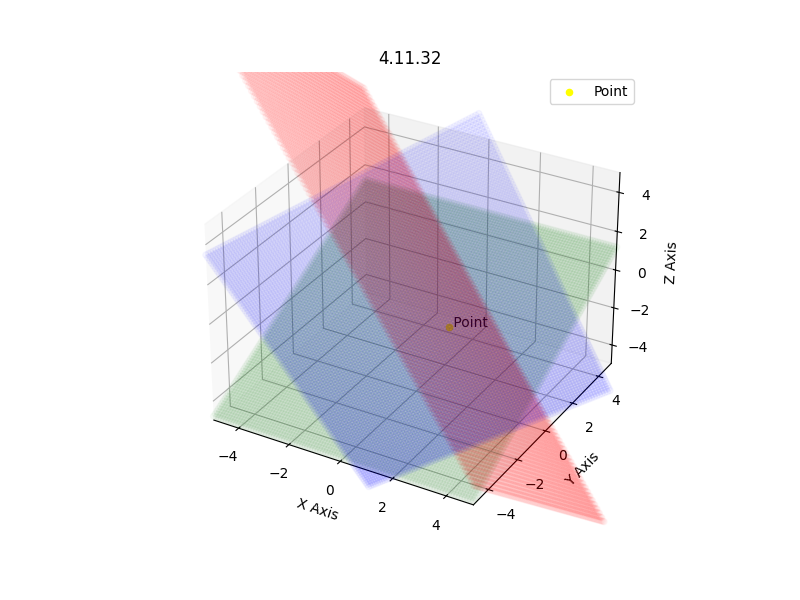
\includegraphics[width=0.8\columnwidth]{../figs/plot.png}
    \caption*{}
    \label{fig:plot}
\end{figure}
\end{frame}

\section{C Code}

\begin{frame}[fragile]{C code for generating points on plane}
\begin{lstlisting}[language=C]
 void generate_plane_points(
    // Output params
    double* x_coords, double* y_coords, double* z_coords,
    // Grid params
    double x_min, double x_max, int x_steps,
    double y_min, double y_max, int y_steps,
    // Plane stuff
    double n1, double n2, double n3, double c) {
    double x_step_val = (x_max - x_min) / (x_steps - 1);
    double y_step_val = (y_max - y_min) / (y_steps - 1);
    int index = 0;
    for (int i = 0; i < x_steps; i++) {
        for (int j = 0; j < y_steps; j++) {
            double current_x = x_min + i * x_step_val;
            double current_y = y_min + j * y_step_val;
            double current_z;
\end{lstlisting}
\end{frame}
\begin{frame}[fragile]
 \begin{lstlisting}[language=C]
            // Vertical plane check
            if ((c < 1e-9)&&(c > -1e-9)) {
                current_z = 0.0;
            } else {
                current_z = (-n1 * current_x - n2 * current_y + c) / n3;
            }
            x_coords[index] = current_x;
            y_coords[index] = current_y;
            z_coords[index] = current_z;
            index++;
        }
    }
}
 \end{lstlisting}
\end{frame}

\section{Python Code}
\subsection{Using shared objects}
\begin{frame}[fragile]{Python code for plotting using C}
\begin{lstlisting}[language=Python]
import ctypes
import numpy as np
import numpy.linalg as LA
import matplotlib.pyplot as plt
from mpl_toolkits.mplot3d import Axes3D

e1 = np.array([2, 1, 1, 1])
e2 = np.array([1, -2, -1, 3 / 2])
e3 = np.array([0, 3, -5, 9])


cols = ["red", "blue", "green"]
\end{lstlisting}
\end{frame}
\begin{frame}[fragile]
 \begin{lstlisting}[language=Python]
lib = ctypes.CDLL("./plane.so")

lib.generate_plane_points.argtypes = [
    ctypes.POINTER(ctypes.c_double),
    ctypes.POINTER(ctypes.c_double),
    ctypes.POINTER(ctypes.c_double),
    ctypes.c_double,
    ctypes.c_double,
    ctypes.c_int,
    ctypes.c_double,
    ctypes.c_double,
    ctypes.c_int,
    ctypes.c_double,
    ctypes.c_double,
    ctypes.c_double,
    ctypes.c_double,
]
lib.generate_plane_points.restype = None
 \end{lstlisting}
\end{frame}
\begin{frame}[fragile]
 \begin{lstlisting}[language=Python]
fig = plt.figure(figsize=(8, 6))
ax = fig.add_subplot(111, projection="3d")

x_steps, y_steps = 100, 100
total_points = x_steps * y_steps
x_plane = np.zeros(total_points, dtype=np.double)
y_plane = np.zeros(total_points, dtype=np.double)
z_plane = np.zeros(total_points, dtype=np.double)
 \end{lstlisting}
\end{frame}
\begin{frame}[fragile]
 \begin{lstlisting}[language=Python]
for i in range(1, 4):
    lib.generate_plane_points(
        x_plane.ctypes.data_as(ctypes.POINTER(ctypes.c_double)),
        y_plane.ctypes.data_as(ctypes.POINTER(ctypes.c_double)),
        z_plane.ctypes.data_as(ctypes.POINTER(ctypes.c_double)),
        -5.0,
        5.0,
        x_steps,
        -5.0,
        5.0,
        y_steps,
        eval(f"e{i}")[0],
        eval(f"e{i}")[1],
        eval(f"e{i}")[2],
        eval(f"e{i}")[3],
    )
    ax.scatter(x_plane, y_plane, z_plane, alpha=0.03, color=cols[i - 1])
 \end{lstlisting}
\end{frame}
\begin{frame}[fragile]
 \begin{lstlisting}[language=Python]
ax.scatter(1, 1 / 2, -3 / 2, color="yellow", label="Point")
ax.text(1, 1 / 2, -3 / 2, " Point")

ax.set_xlabel("X Axis")
ax.set_ylabel("Y Axis")
ax.set_zlabel("Z Axis")
ax.set_title("4.11.32")
ax.set_xlim([-5, 5])
ax.set_ylim([-5, 5])
ax.set_zlim([-5, 5])
ax.legend()
ax.grid(True)

plt.savefig("../figs/plot.png")
plt.show()
 \end{lstlisting}
\end{frame}
\subsection{Plot}
\begin{frame}{Plot}
 \begin{figure}[H]
    \centering
    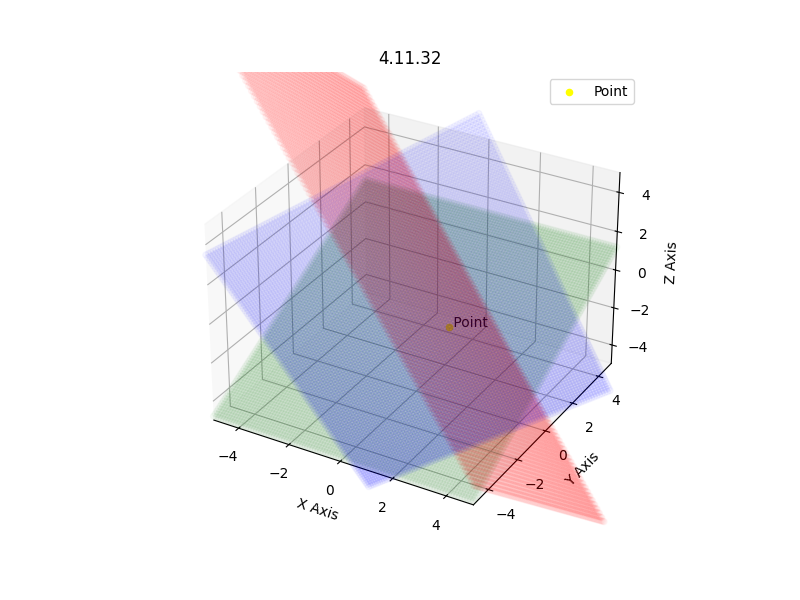
\includegraphics[width=0.8\columnwidth]{../figs/plot.png}
    \caption*{}
    \label{fig:plot}
\end{figure}
\end{frame}
\subsection{In pure Python}
\begin{frame}[fragile]{Pure Python code}
 \begin{lstlisting}[language=Python]
import numpy as np
import numpy.linalg as LA
import matplotlib.pyplot as plt
from mpl_toolkits.mplot3d import Axes3D
e1 = np.array([2, 1, 1, 1])
e2 = np.array([1, -2, -1, 3 / 2])
e3 = np.array([0, 3, -5, 9])
cols = ["", "red", "blue", "green"]
fig = plt.figure(figsize=(8, 8))
ax = fig.add_subplot(111, projection="3d")
x, y = np.meshgrid(range(-10, 10), range(-10, 10))
for i in range(1, 4):
    z = (
        -(eval(f"e{i}")[0] * x + eval(f"e{i}")[1] * y - eval(f"e{i}")[3])
        / eval(f"e{i}")[2]
    )
    ax.plot_surface(x, y, z, alpha=0.35, color=cols[i])
 \end{lstlisting}
\end{frame}
\begin{frame}[fragile]{Pure Python code}
 \begin{lstlisting}[language=Python]
ax.scatter(1, 1 / 2, -3 / 2, color="yellow", label="Point")
ax.text(1, 1 / 2, -3 / 2, " Point")

ax.set_xlabel("X-axis")
ax.set_ylabel("Y-axis")
ax.set_zlabel("Z-axis")
ax.set_title("5.2.57")
ax.set_xlim([-10, 10])
ax.set_ylim([-10, 10])
ax.set_zlim([-10, 10])
ax.legend()
ax.grid(True)

plt.savefig("../figs/python.png")
plt.show()
 \end{lstlisting}
\end{frame}
\subsection{Plot}
\begin{frame}{Plot}
 \begin{figure}[H]
    \centering
    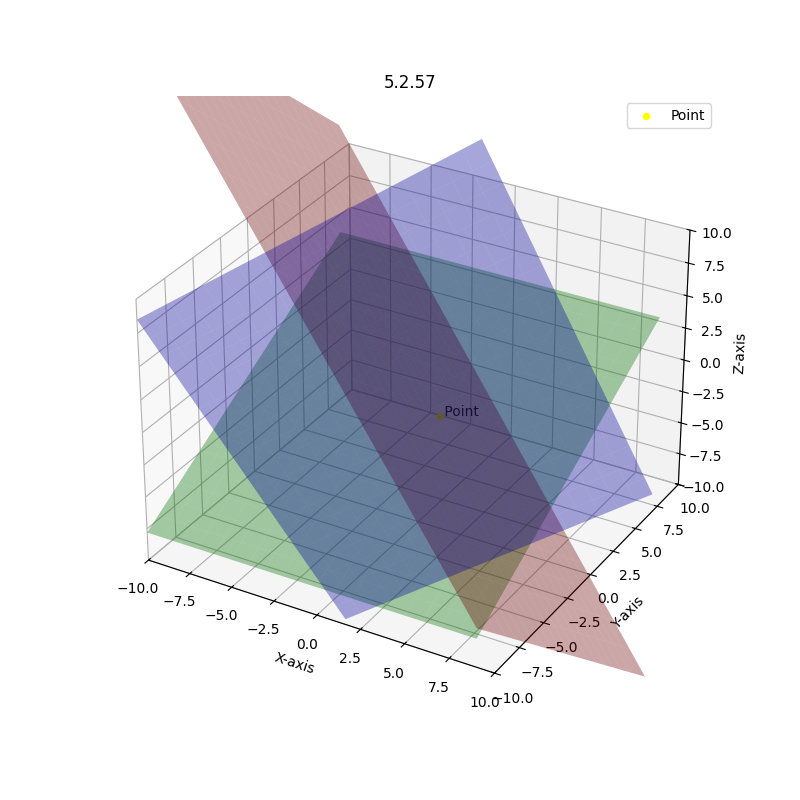
\includegraphics[width=0.75\columnwidth]{../figs/python.png}
    \caption*{}
    \label{fig:plot}
\end{figure}
\end{frame}
\end{document}
